\begin{table}[h]
\centering
\label{data_sources}
\caption{Origins of labeled training data}
\begin{tabular}{|r|r|l|}
\hline
Amount & Label & Origin \\ \hline
9 & DATA & Manual Google search for Open Data
repositories \\ \hline
82 & DATA & Repositories of GitHub user `datasets' \\ \hline
17 & EDU & GitHub Search for ``course, material'' \\ \hline
17 & DOCS & GitHub Search for ``documentation'' \\ \hline
423 & WEB & Google Search for ``site:.github.io'' \\ \hline
58 & HW & GitHub Search for ``homework, assignments,
solution'' \\ \hline
13 & DEV & Showcases ``Virtual Reality'' \\ \hline
12 & DEV & Showcases ``Software Development Tools'' \\ \hline
14 & DEV & Showcases ``Front-end JavaScript frameworks'' \\ \hline
20 & DEV & Showcases ``DevOps tools'' \\ \hline
16 & DEV & Showcases ``Text editors'' \\ \hline
24 & DEV & Showcases ``Game Engines'' \\ \hline
27 & DEV & Showcases ``Web Application Frameworks'' \\ \hline
42 & DEV & Showcases ``Programming Languages'' \\ \hline
180 & DOCS & GitHub Repo Content: awesome-awesomeness \\ \hline
6 & DATA & Showcases ``Open Data'' \\ \hline
86 & HW & Github Search for ``homework, solution'' \\ \hline
\end{tabular}
\end{table}

\begin{figure}[h]
	\centering
		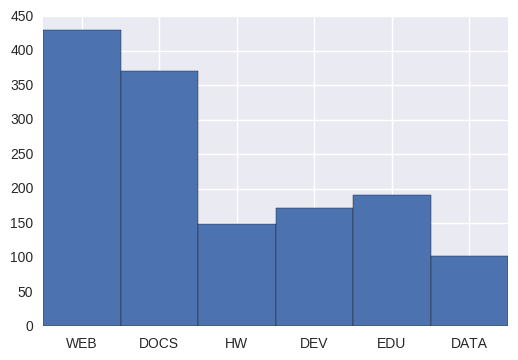
\includegraphics[width=10cm]{graphics/training_data_distribution.png}
	\caption{Training Data Distribution}
	\label{training_data_distribution}
\end{figure}


\begin{figure}[h]
	\centering
		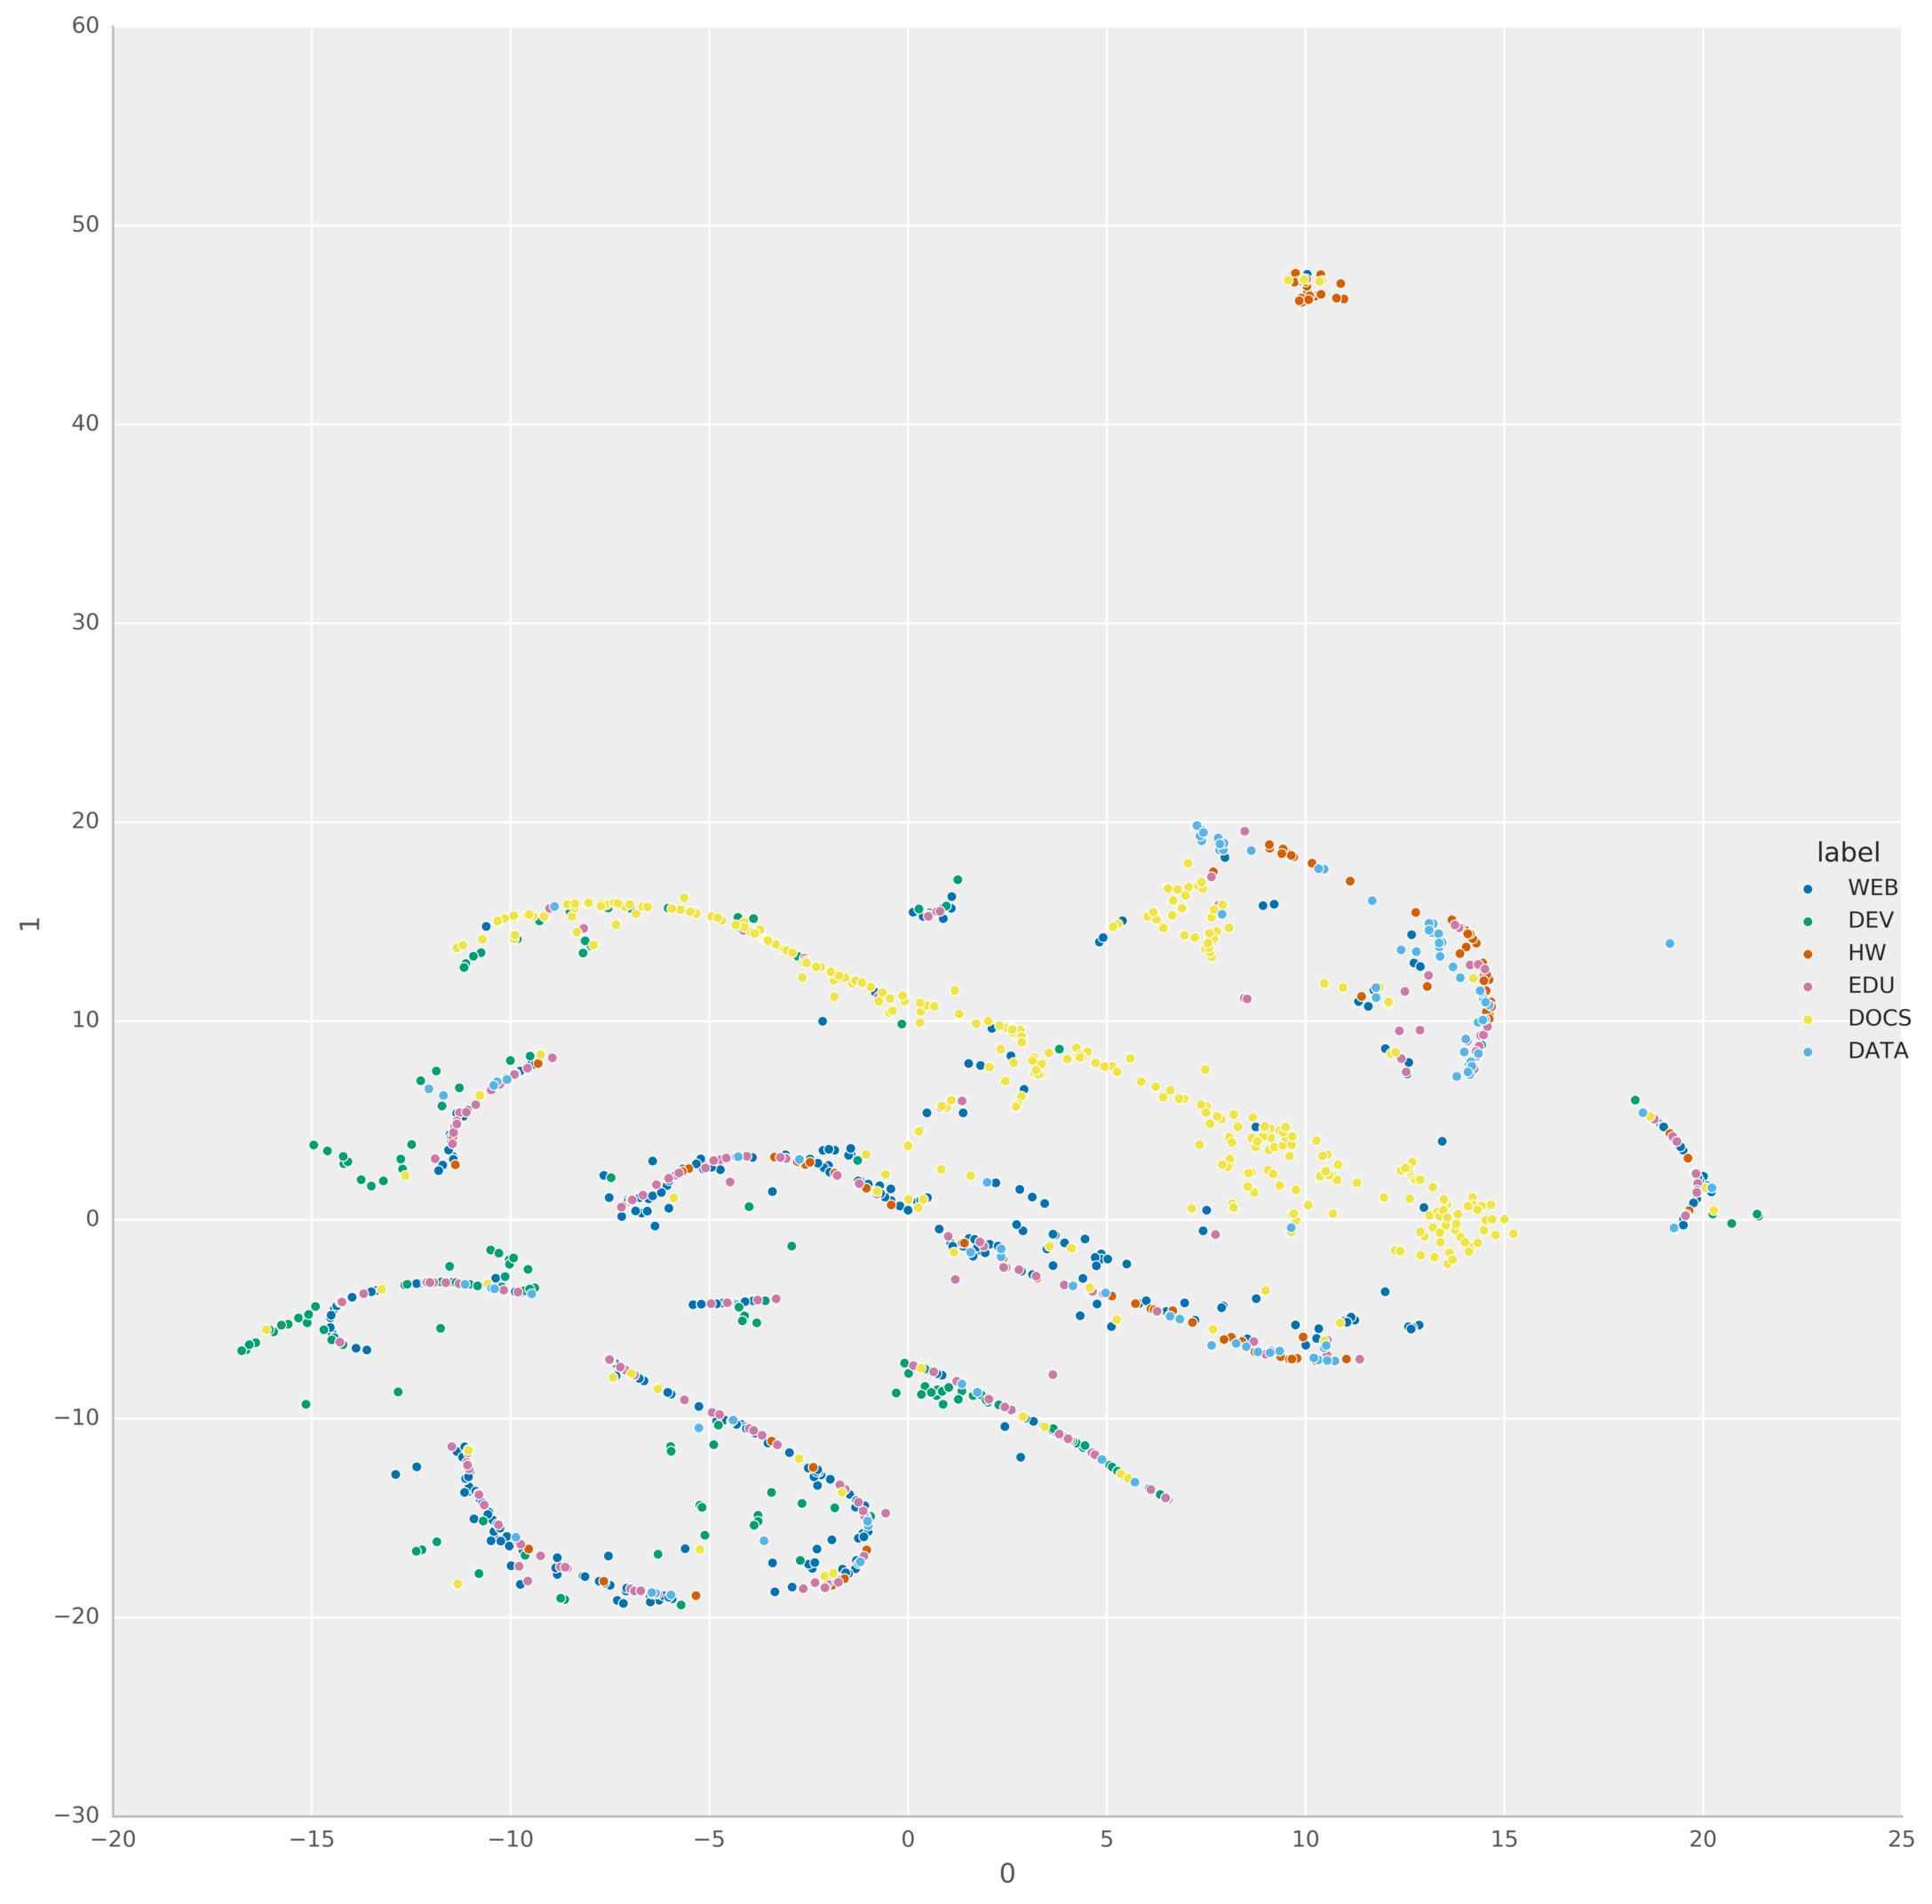
\includegraphics[width=18cm]{graphics/t-sne-training-data.png}
	\caption{Distribution of the labeled data entries using t-SNE}
	\label{t-sne-training-data}
\end{figure}


\begin{figure}[h]
	\centering
		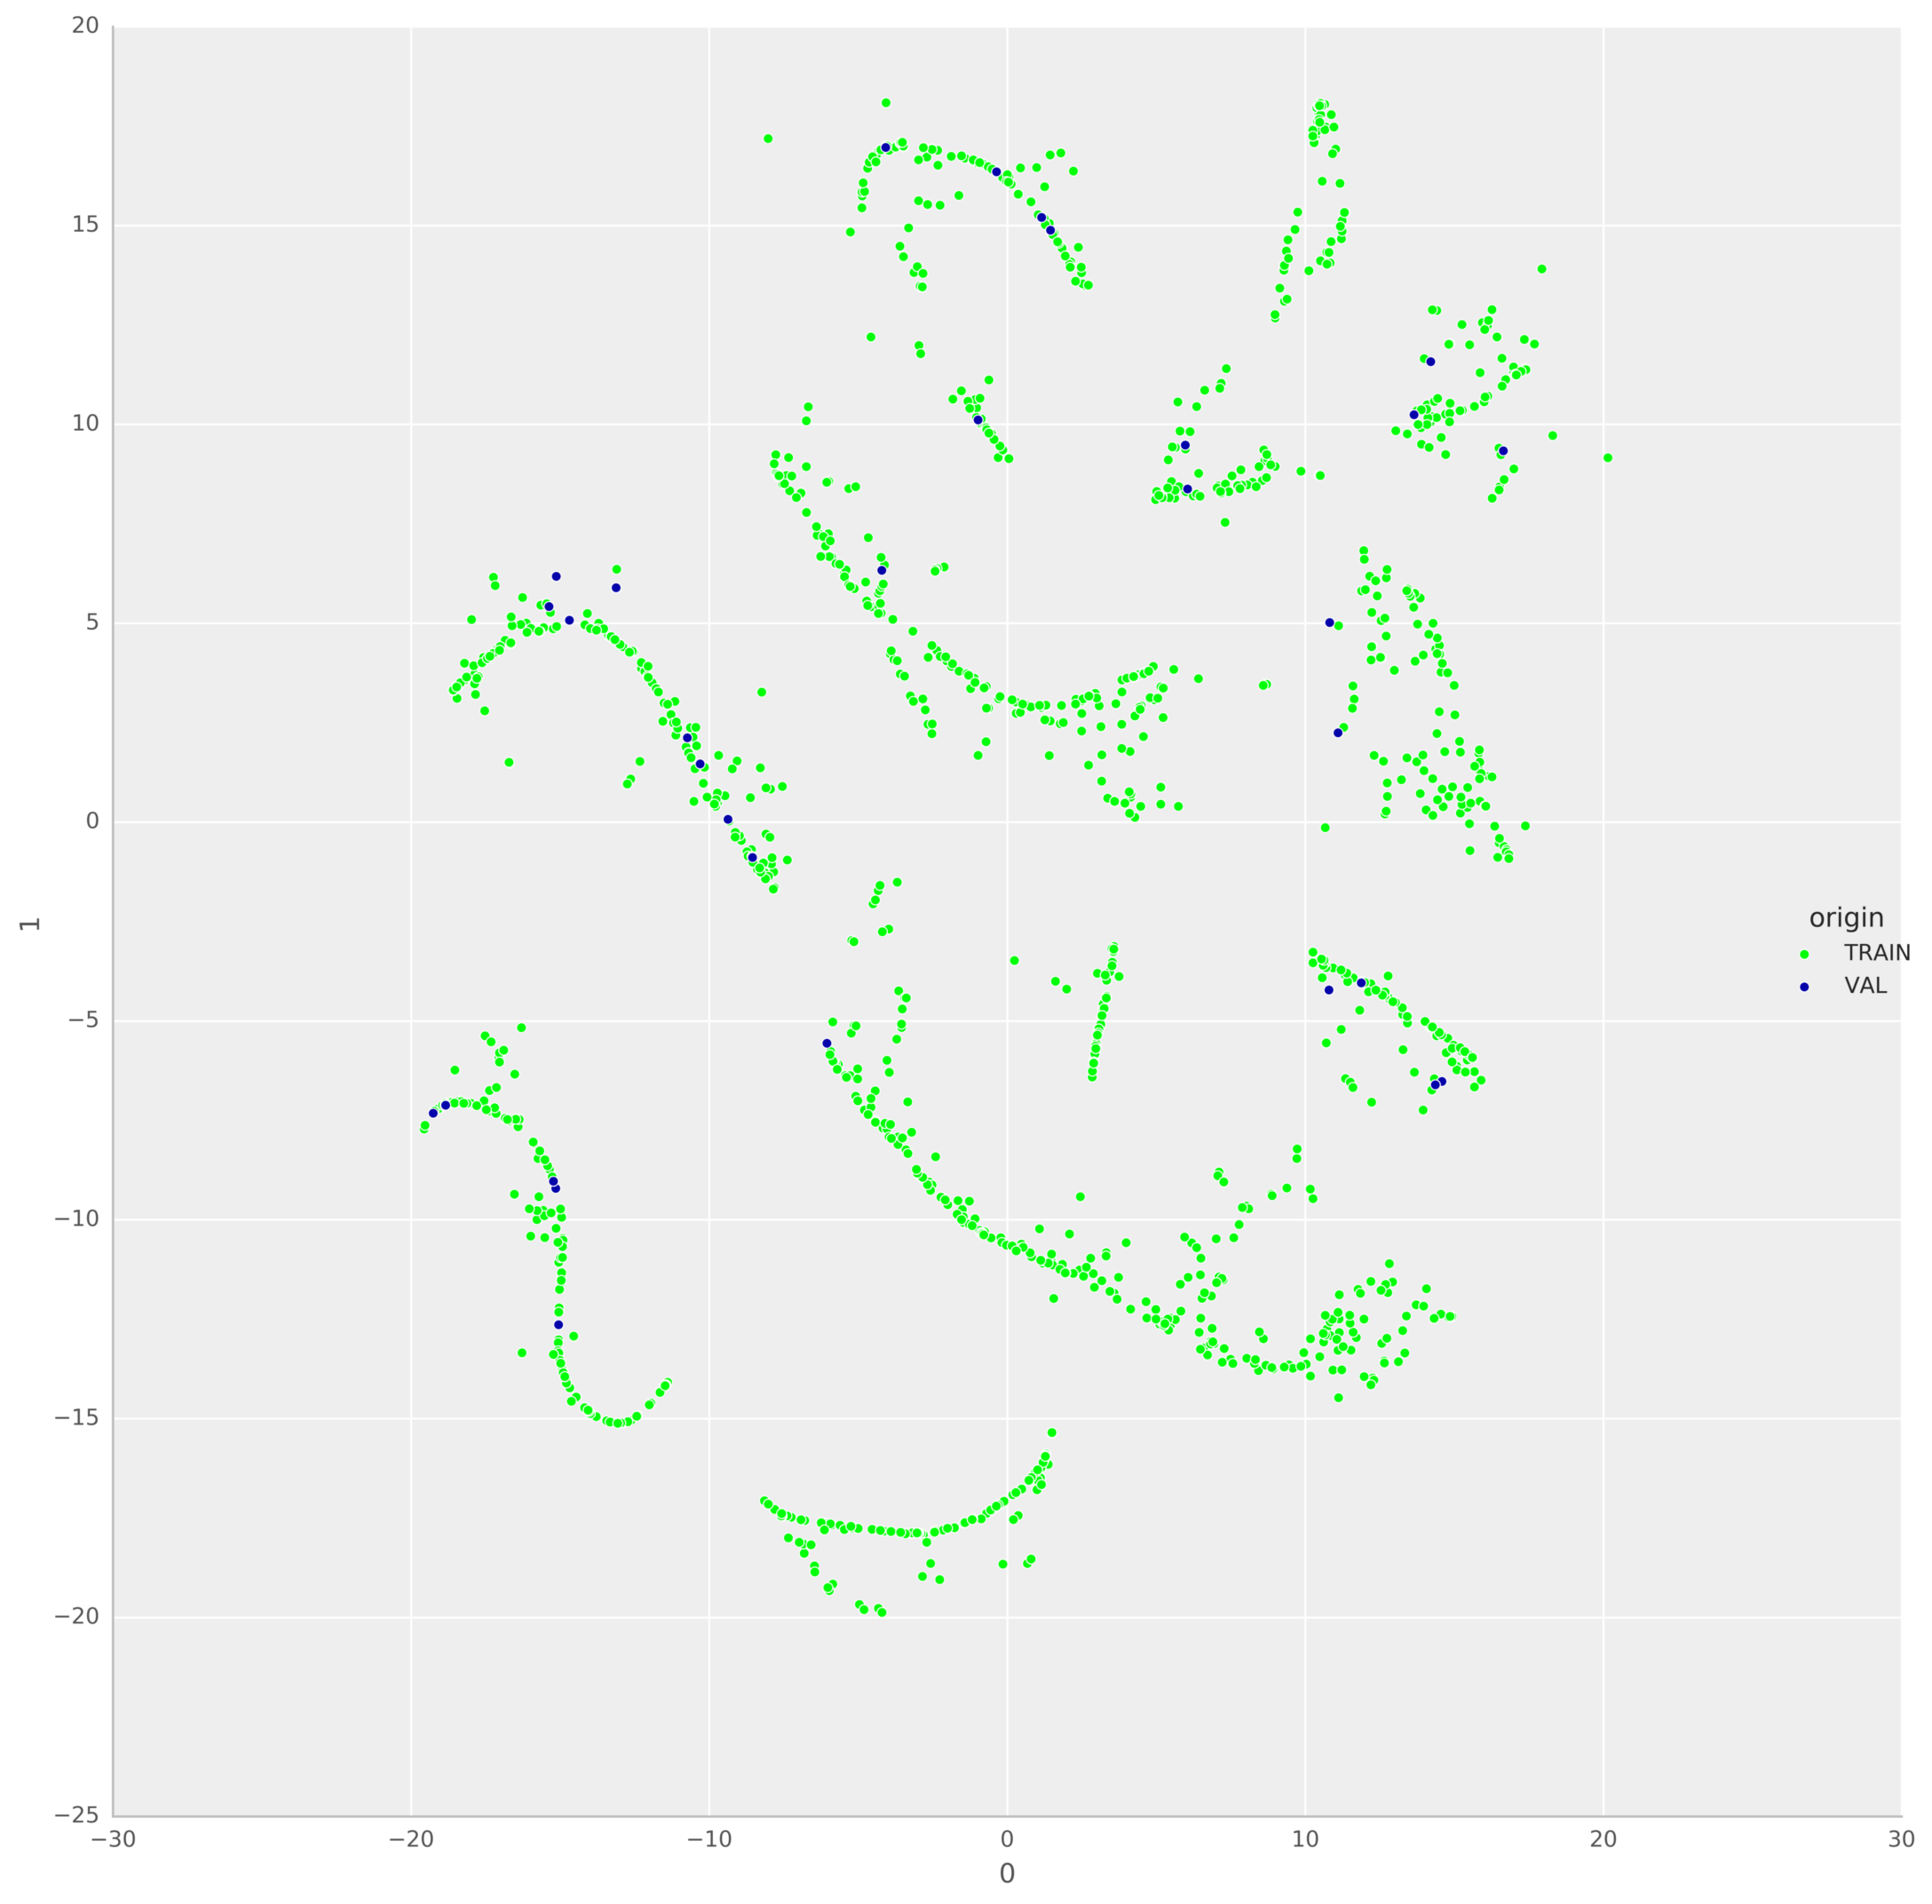
\includegraphics[width=18cm]{graphics/t-sne-validation-data.png}
	\caption{Distribution of the validation data entries using t-SNE}
	\label{t-sne-validation-data}
\end{figure}

\begin{table}[h]
\centering
\caption{Numeric Features}
\label{features}
\begin{tabularx}{\linewidth}{|l|X|}
\hline
Feature Name           & Description                                                                        \\ \hline
watchers               & Number of users who get notifications about the repo                               \\ \hline
mentionableUsers       & Number of mentionable users (collaborators, contributors, ...)                     \\ \hline
open\_pull\_requests   & Number of open pull requests                                                       \\ \hline
closed\_pull\_requests & Number of closed pull requests                                                     \\ \hline
merged\_pull\_requests & Number of merged pull requests                                                     \\ \hline
open\_issues           & Number of open issues                                                              \\ \hline
closed\_issues         & Number of closed issues                                                            \\ \hline
forks                  & Number of forks                                                                    \\ \hline
stargazers             & Number of users who "starred" the repo                                             \\ \hline
projects               & Number of projects (integrated project management tool)                            \\ \hline
size                   & Size of the source code in kilobyte                                                \\ \hline
isOwnerHomepage        & Is the name of the repo REPO\_OWNER.github.io or REPO\_OWNER.github.com?           \\ \hline
hasHomepage            & Does the website \newline{}REPO\_OWNER.github.io/REPO\_NAME exist?                 \\ \hline
hasLicense             & Does the repo have a license file?                                                 \\ \hline
hasTravisConfig        & Does the repo have a Travis configuration file?                                    \\ \hline
hasCircleConfig        & Does the repo have a CircleCI configuration file?                                  \\ \hline
hasCiConfig            & hasTravisConfig OR hasCircleConfig                                                 \\ \hline
commitsCount           & Number of commits                                                                  \\ \hline
branchesCount          & Number of branches                                                                 \\ \hline
tagsCount              & Number of tags                                                                     \\ \hline
releasesCount          & Number of releases                                                                 \\ \hline
LANGUAGE\_*            & How much code was written in the language in percent (e.g. LANGUAGE\_Python, ...) \\ \hline
\end{tabularx}
\end{table}

\begin{figure}[h]
	\centering
		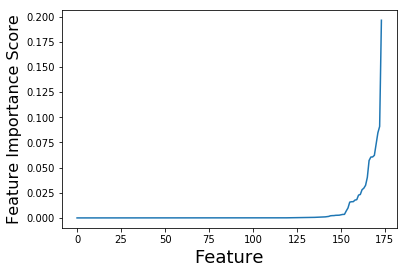
\includegraphics[width=12cm]{graphics/feature_importance_numeric.png}
	\caption{Feature Importance Scores for Numeric Features}
	\label{feature_importance_numeric_graphic}
\end{figure}

\begin{table}[h]
	\centering
	\caption{Top 20 Most Important Numeric Features}
	\label{feature_importance_numeric}
	\begin{tabular}{|l|l|l|l|}
	\hline
		Feature Names & Scores & Feature Names & Scores \\ \hline
		isOwnerHomepage  &   0.1793 & hasHomepage & 0.1297 \\ \hline
		stargazers  &   0.0726 & mentionableUsers & 0.0642 \\ \hline
		size  &   0.0581 & watchers & 0.0561 \\ \hline
		commitsCount  &   0.0492 & closed\_issues & 0.0415 \\ \hline
		merged\_pull\_requests  &   0.0389 & open\_issues & 0.0379 \\ \hline
		forks  &   0.0376 & closed\_pull\_requests & 0.0368 \\ \hline
		tagsCount  &   0.0245 & branchesCount & 0.0239 \\ \hline
		hasTravisConfig  &   0.0235 & open\_pull\_requests & 0.0223 \\ \hline
		releasesCount  &   0.0214 & hasLicense & 0.0148 \\ \hline
		hasCiConfig  &   0.0124 & LANGUAGE\_Python & 0.0090 \\ \hline
	\end{tabular}
\end{table}

\begin{table}[h]
	\label{benchmark_numeric}
	\centering
	\caption{Accuracies on the given validation data and additional validation data}
	\begin{tabular}{|r|r|r|r|r|r|r|r|}
	\hline
	          & Naive Bayes & Tree & Forest & k-NN & SVM & Gradient Boost & Ensemble \\ \hline
	Validation& 40\%        & 35\%          & 42\%          & 25\% & 25\% & 41\% & 45\%         \\ \hline
	Add. Val. & 19\%        & 21\%          & 23\%          & 21\% & 20\% & 22\% & 25\%         \\ \hline
	\end{tabular}
\end{table}

\begin{figure}[h]
	\centering
		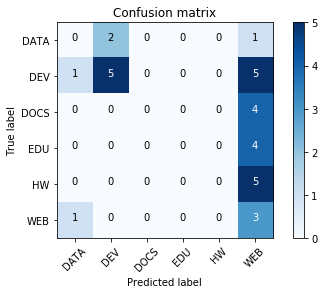
\includegraphics[width=8cm]{graphics/confusion-matrix-numeric-ensemble.png}
	\caption{Confusion Matrix for Numeric Ensemble (46\% Accuracy)}
	\label{confusion_matrix_numeric_ensemble}
\end{figure}

\begin{table}[h]
\centering
\caption{Boolean Matrix for Numeric Ensemble}
\label{boolean_matrix_numeric_ensemble}
\begin{tabular}{|r|r|r|r|r|}
 \hline
 Label & Predicted Correctly & Predicted Incorrectly & Precision & Recall \\ \hline
 WEB & 3 & 1 & 0.14 & 0.75 \\ \hline
 DOCS & 0 & 4 & 0.00 & 0.00 \\ \hline
 HW & 0 & 5 & 0.00 & 0.00 \\ \hline
 DEV & 5 & 6 & 0.71 & 0.45 \\ \hline
 EDU & 0 & 4 & 0.00 & 0.00 \\ \hline
 DATA & 0 & 3 & 0.00 & 0.00 \\ \hline
 \multicolumn{3}{|l|}{Weighted Average} & 0.27 & 0.26 \\ \hline
 \end{tabular}
 \end{table}
